%!TEX root = ../thesis.tex

\chapter{理论模型}
\label{modelselection}
\section{微观层次}
迄今为止我国尚未发生类似金融危机时的大片企业集中倒下,违约更多是非系统性风险造成的,绝大多数违约都是公司层面发生了一些问题导致的。因此本文的分析重点将集中在微观层次
本文将微观层面影响企业违约的因素分为以下四类,主要包含企业层面的指标:
\subsection{公司层面}

国企发行了80\%的债券,但违约中只占了15\%,有学者指出,这可能是由于国企存在政府支持\cite{mo2021china},市场上打破“刚兑信仰”后的确有过“国企信仰”和“城投信仰”;也有可能是国企通常相对资金雄厚,经营情况较好。因此,本文将公司性质作为影响因素之一纳入后续建模中。
同样的,上市企业比非上市企业融资方式更多,融资额往往也更大,某些违约企业也认为其违约原因是上市失败,因此上市与否或许也可能影响违约。

股东对企业的支持对于企业是否能安全度过难关非常重要,如苏宁易购实控人地位不保之后,在企业危难时众股东自扫门前雪,没有人愿向企业注血,最终苏宁走向违约。通常而言大股东持股比例越高,对企业的重视程度会越大,更有可能为了避免违约后其持有的大量股权价值归零而为企业提供资金支持或豁免债务。

此外,正如\ref{sec:zs}中众多学者对公司治理的研究所揭示,公司治理成效也可能是影响违约的因素。但是,一方面公司治理会影响违约与否,另一方面违约企业通常会面临法律纠纷、债权人接管等情况,令企业公司治理发生很大变化,二者存在双向因果。
本文以持有基金占比作为公司治理的代理变量。
债券持有者大多为银行、信托或公募基金(含券商资管),二者差别之一是换手率:银行、信托申购债券后通常会持有至债券到期,而公募基金则会假设可能需要卖出。这是因为银行的资金基本不需要考虑赎回的压力,只需要考虑期限与负债匹配,信托投资期限与标的在合同中有规定,而公募基金则需要防止净值下跌引发赎回潮。因此公募基金不仅关注利息与本金的给付,还关心债券估值变动带来的资本利得。
由于担心债券在持有期间贬值,公募基金更会担心企业公司治理存在问题。
如果公司治理水平低,债券潜在的下跌可能性更大\Parencite{anginer2018corporate};实务中其亦会关注企业的高管行为。即基金持有比例和公司治理强相关。
公募基金在评级下调超出阈值后必须斩仓,但评级下调的债券中违约终究只是少数,因此公募基金持有比例与违约弱相关,现实中亦有基金公司“踩雷”华夏幸福等的违约债券。因此本文计划采用基金持有比例来表征公司治理的好坏。

最后,公司层面还有一些难以量化的因素,如发行人主观意愿(花样年地产账面现金充足“花式”躺平违约 \footnote{\url{https://company.stcn.com/gsxw/202110/t20211005_3737004.html}})、财务造假(五洋建设欺诈发行 \footnote{\url{https://company.stcn.com/gsxw/202101/t20210102_2694254.html}})。但因此违约的终是少数,绝大多数地产商苦苦挣扎避免躺平,绝大多数企业报表准确。因此本文不将这些因素纳入考虑。
\subsection{经营层面}
企业之所以面临流动性危机,很多情况下是经营不及预期、营收大幅亏损,如原“超日太阳”在连续三年大额亏损后,最终无法兑付利息,成为打破刚兑的第一例违约。

在经营层面,客户集中度过高,可能会导致企业面临较高的风险\cite{王雄元2017客户集中度与公司债二级市场信用利差}。集中的客户有能力要求企业降价、使用商票结算等以降低自身成本,以获得更大利润空间。例如建设承包商南通三建,其持有大量恒大商票得不到兑付,流动性告急不得不寻求债务展期。

经营过程中的杠杆率也有可能影响违约\cite{王永钦2019杠杆率如何影响资产价格},如以“高杠杆-高周转”著称的恒大,在融资受限时高杠杆的游戏进行不下去,债务难以接续进而违约。但一方面很多违约公司会美化负债率,用诸如战略投资者等明股实债的方式,尽各种手段将负债隐藏到表外;另一方面,不同性质的行业杠杆差异较大,如重工业和服务业之间相似的负债率并不意味着相近的爆仓的可能性,简单比较负债率并不可取。基于此本文不采用资产负债表科目刻画杠杆率,而是采用标准券折算率这一比较市场化的指标,即质押企业债券可以获得多大比例的标准券来衡量企业杠杆率。折算率高意味着市场允许企业股东可以通过质押他持有的债券的方式撬动更多融资,即增加杠杆。

\subsection{财务层面}
对于会计指标,\Textcite{blochlinger2018ratings}发现以美国债券市场发行人作为研究对象, Altman's Z 指标是一个比较综合的、很好的预测违约的会计指标。因此本文尝试引入 Z 值作为综合的财务指标。

此外,违约本质上是企业持有的现金及其等价物无法偿还到期债务,但也存在一定的可能,即公司虽然遇到短期流动性危机,但未来长期表现还是有可能转好,如盐湖股份短期流动性告急,通过银行等机构的债转股使其资产不至于低价贱卖流失,重整两年后成为锂矿龙头。因此本文也将考虑现金短债比这一因素。

\subsection{评级指标}
信用评级是企业违约风险的直观表述,但我国信用评级市场尚不完善,存在一定的评级结果虚高情况,
如图\ref{fig:rating}所示,新发行债券有一半为最高评级 AAA 。
\begin{figure}[ht]
	\centering
	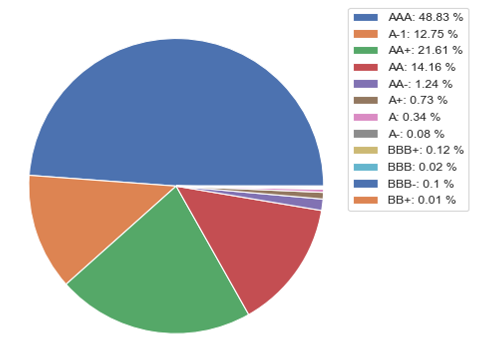
\includegraphics[width=0.9\linewidth]{./data/rating_from_2014.png}
	\caption{\label{fig:rating}信用债发行评级统计}
\end{figure}


虽然以预测的角度看评级并不完全准确,但以后验的角度看,评级也反映了一定的公开与非公开信息,因此本文也将主体评级纳入考虑。

尽管有研究指出,相比于评级,债券交易的价格可能更有效\cite{badoer2019relevance}。我国也是如此,债券价格大幅偏离估值往往是违约的先兆,一般认为面值100的债券价格下跌至60元左右相当于即将违约,已经违约的债券往往价格只有20元左右。但单纯以价格异动预测违约存在不少假阳性情况,特别是在城投债中,一些经济欠发达省市的城投债成交收益率有时能达到20\%乃至更高,但至今仍未有城投债违约出现。

\section{中观层次}
中观层次为非企业级、非全国级的因素,如行业、流动性和区位因素等。

行业方面,正如\Textcite{azizpour2018exploring} 指出美国违约企业基本可以排除行业聚类,我国债券违约基本可以排除大多数的行业聚类,即某行业因行业景气集中某段时间违约的情况。看似较高违约率的行业,均是因为单一主体违约余额较大(如方正集团导致计算机行业、华晨汽车导致汽车行业、紫光集团导致电子行业、山东如意导致纺织行业违约率激增),如图  \ref{fig:industry} 所示。
即便是近期的房地产违约风波,也并非主要由于行业景气度,而是由于房地产“三条红线” 等政策约束高杠杆的经营。因此本文将主要考虑房地产政策(房地产行业且时间大于2020 年),而不考虑每个行业本身。
\begin{figure}[ht]
	\centering
	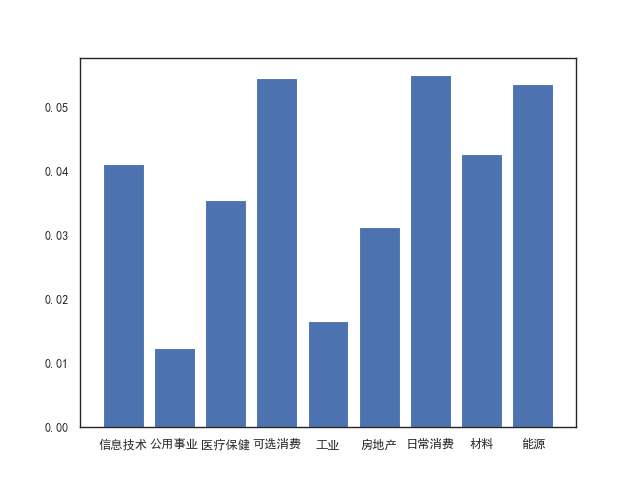
\includegraphics[width=.9\linewidth]{./data/industry.png}
	\caption{\label{fig:industry}违约债分行业分布}
\end{figure}

\begin{figure}[ht]
	\centering
	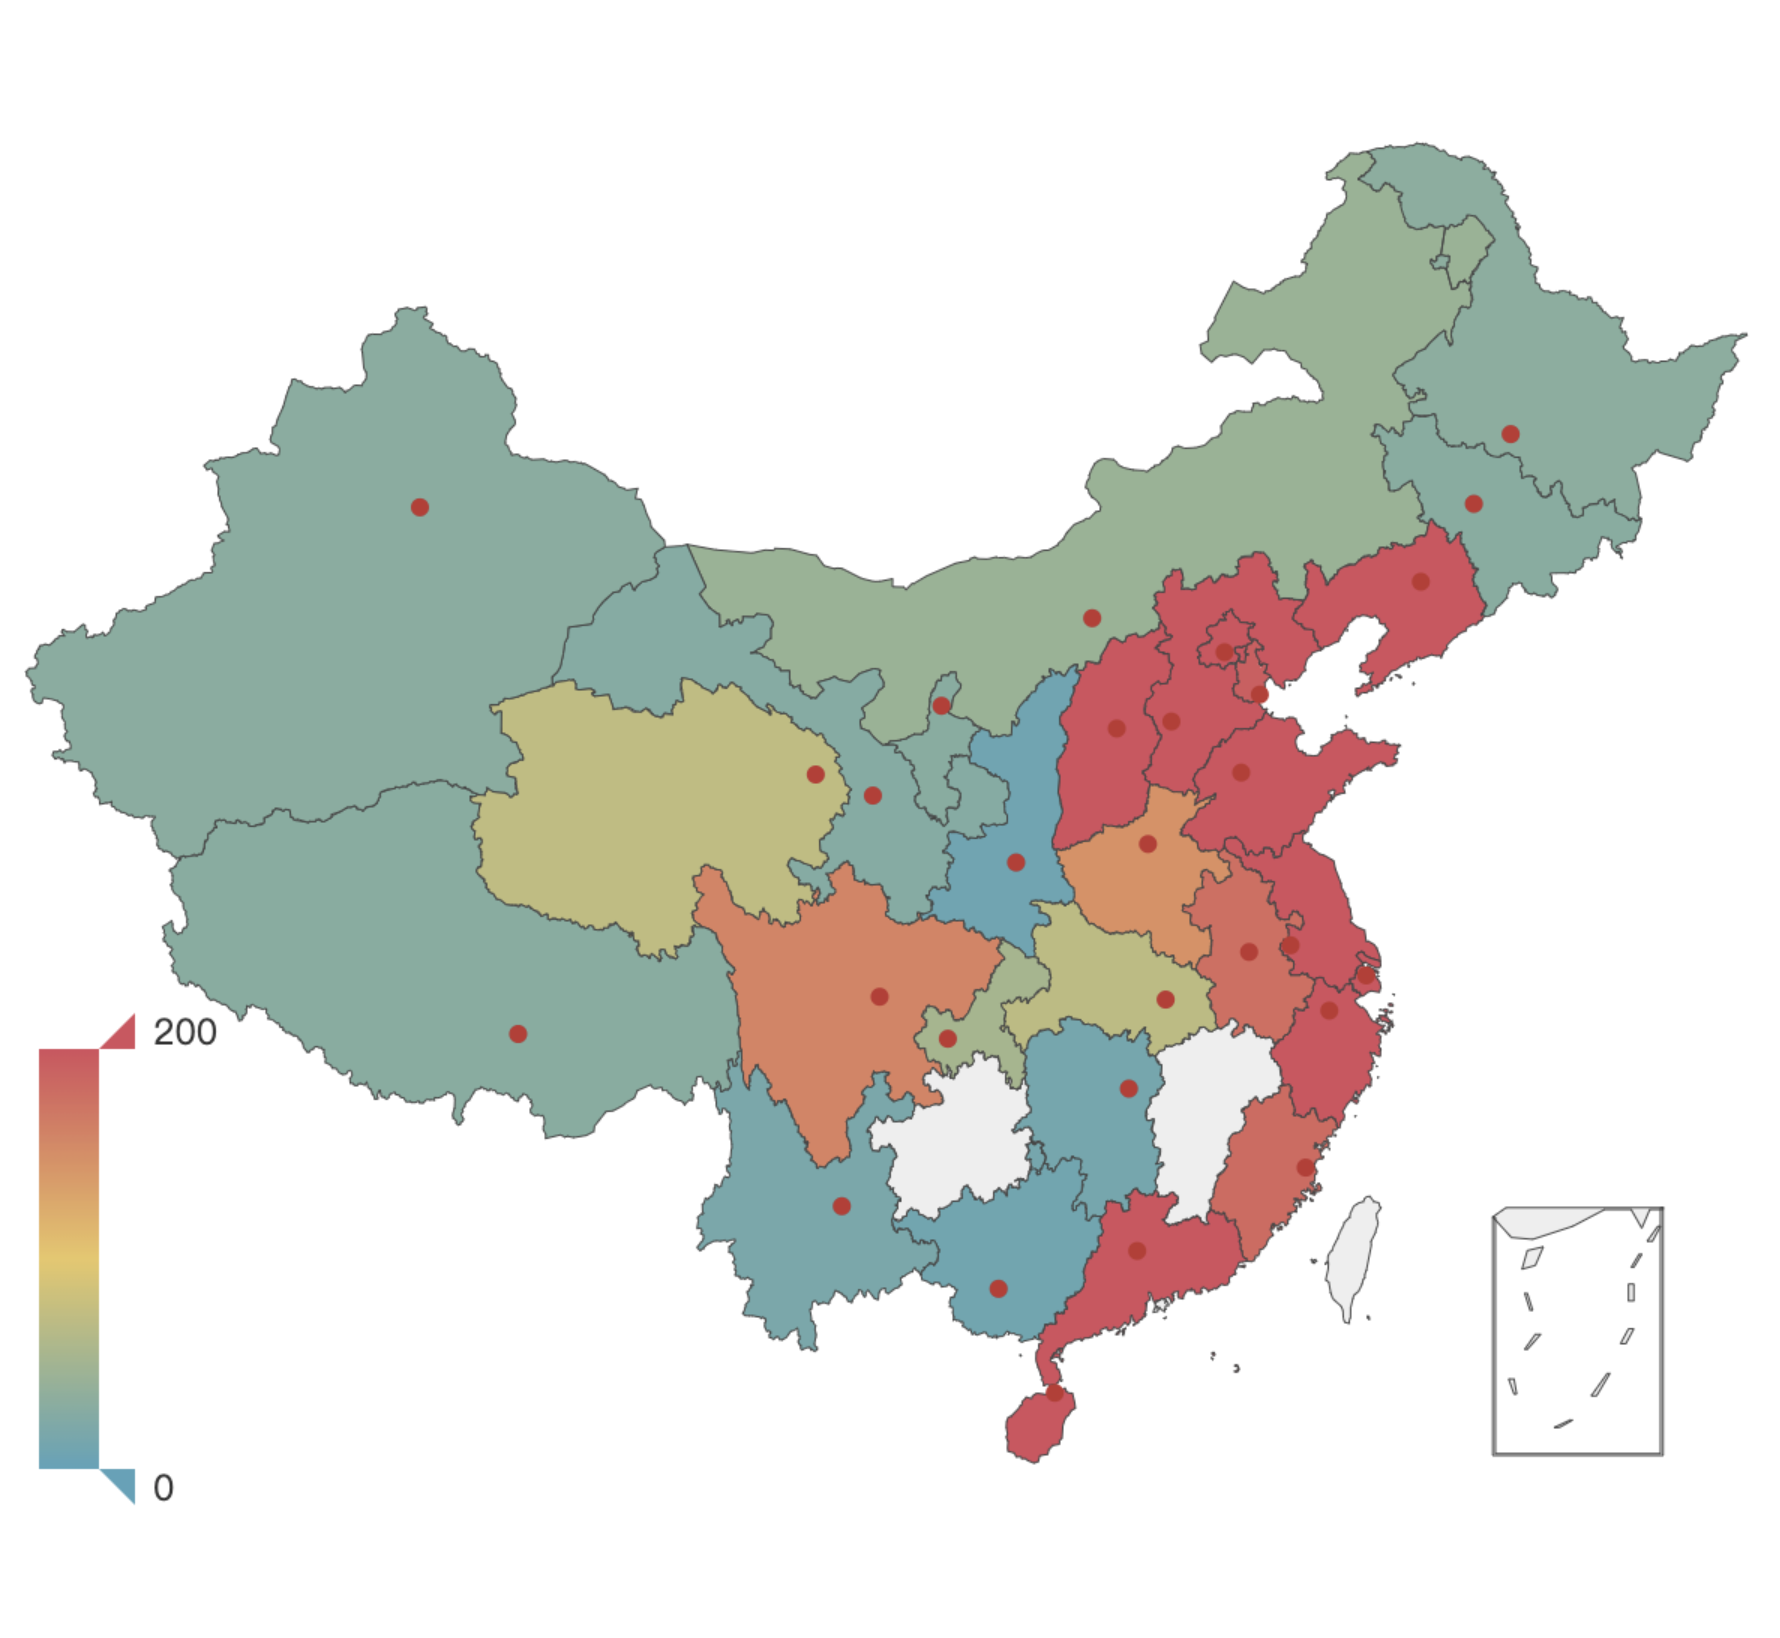
\includegraphics[width=.9\linewidth]{./data/default_by_geo.png}
	\caption{\label{fig:geo}各省违约债累计余额(亿元)}
\end{figure}
区位方面,一方面经济落后地区违约风险较大,另一方面经济较好的地区企业发债数量较多可能导致违约金额较大,如图\ref{fig:geo}显示出后一种作用较强,尽管某些经济欠发 达地区似乎仍然维持刚性兑付。尽管看似部分地区违约率高,但事实上高违约率的原因大多也是单一违约主体违约金额大,如河北的华夏幸福、辽宁的华晨宝马、海南的海航、青海的青国投等等,总的来说地理上的传染尚不明晰。

流动性方面,当市场流动性偏紧时,如永煤违约后风险偏好迅速下降,各机构连 AAA 国企也不敢买,成交量萎靡流动性偏紧,进而导致一级市场上冀中能源、紫光、清华控股等无法发债接续,到期压力巨大, 最终部分企业走向违约。因此,本文计划以市场成交金额作为流动性指标。

\section{宏观层次}
如\ref{sec:zs}中学者研究,货币政策与财政政策可能会对企业违约有影响。学者普遍认为财政政策的挤出效应会增加企业违约,“国进民退”;而货币政策收紧企业可能会面临融资难,进而走向违约,货币政策放松如预期外降准则成为恒大倒下的应对手段。本文计划财政政策使用政府支出占GDP比重表征,货币政策以 SHIBOR 利率表征。

有学者对债券回报率做 Fama 因子分析
\cite{chung2019volatility}
,发现以 VIX 指数为代表的波动风险在债券的回报中是普遍存在的。
高波动性环境下,企业的投资亏损的可能性增加,流动资金缩水,同时企业质押的债券、股票需要补充抵押品。典型的例子是结构化发行爆仓后违约的精功集团。所谓“结构化发行”是指,发行人通过资管产品的分级安排来放大杠杆,自由资金购买劣后级以换取其他资金购买优先级,即“自融”。这就加大了波动性的影响,市场高波动情况下不断增加抵押,爆仓后投资亏损走向违约,我国债券市场如今对这种方式明令禁止。
因此本文效仿选择上证 50 期权的隐含波动率作为波动率指标,2015 年期权推出之前则采用上证历史波动率。
